题意:有n层,有n个点分布在这n层上(一层可以有多个点,也可以有0个)。层与层之间的点可以互相走,权为c。另外还有m条无向边,从某个点到某个点,权为w。求1到n的最短路。 \\
此题的关键在于建图。如果采用朴素建图法,相邻两层的点两两加边,复杂度高达N\^2。如果用下面的这个方法,可以将复杂度降到N。 \\
每层虚拟出来两个点,入点和出点。像图中所示连接(省略了m条给定的边)。黑线的权都为0,红线权为c。这样借助两个点,可以实现层与层连接。 \\
一开始想只用一个点,但是这样的话同一层的点就可以通过权为0的路连接起来了。 \\
(后来发现图中最下面少画了一条边……) \\
\begin{center}
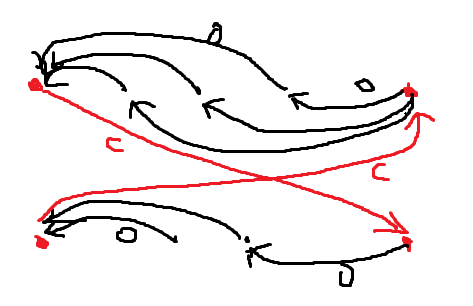
\includegraphics[scale=1]{./模板/13_一些题目/3.jpg}
\end{center}
